\documentclass[12pt,fleqn]{article}
\setlength{\parindent}{0pt}
\usepackage{graphicx}
\usepackage{listings}
\usepackage[latin5]{inputenc}
\setlength{\parskip}{8pt}
\setlength{\parsep}{0pt}
\setlength{\headsep}{0pt}
\setlength{\topskip}{0pt}
\setlength{\topmargin}{0pt}
\setlength{\topsep}{0pt}
\setlength{\partopsep}{0pt}
\setlength{\mathindent}{0cm}

\begin{document}
MIT OCW Cok Degiskenli Calculus - Ders 7

Bugunun konusu ``hersey''. Simdiye kadar gordugumuz her sey
yani. Vektorleri gorduk, noktasal carpimlari (dot product) gorduk. Iki
vektorun noktasal carpimi

\[ \vec{A} \cdot \vec{B} = \sum a_ib_i\]

yani o vektorlerin tum elemanlarinin sirasiyla birbiriyle carpilip
toplanmasi. O da suna esit

\[ = |\vec{A}||\vec{B}|cos \ \theta \]

Noktasal carpimi acilari olcmek icin kullanabiliriz, eger $cos \ \theta$
terimini tek basina birakirsak, geri kalanlari cozeriz. Bu sekilde iki
vektorun dik olup olmadigini da anlariz. Cunku o zaman sonuc sifir olur, ve
$cos \ \theta = 0$ ise aci dik demektir. 

Gordugumuz bir diger kavram capraz carpim (cross product) kavramiydi. 

\[ \vec{A} \times \vec{B} = 
\left|\begin{array}{rrr}
\vec{i} & \vec{j} & \vec{k}  \\
a_1 & a_2 & a_3 \\
b_1 & b_2 & b_3 
\end{array}\right|
\]

Esitligin sagindaki determinant isareti, matris isareti degil, buna
dikkat. Capraz carpimin uygulamalari uzayda bir ucgenin alanin bulmak
mesela. 

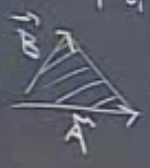
\includegraphics[height=2cm]{7_1.png}

Bu alan

\[ \frac{1}{2}|\vec{A} \times \vec{B}| \]

ile hesaplanir. Cunku $|\vec{A} \times \vec{B}|$ bir paralelogram verir,
onun yarisi aradigimiz ucgenin alanidir.

Capraz carpimin bir diger uygulama alani iki vektore ayni anda dik olan
ucuncu bir vektoru bulmaktir. Ona baglantili olarak bir duzleme (plane) dik
olan bir vektoru bulmak, yani ``normal vektoru'' bulmak. Duzlemin formulu
nedir? 





\end{document}
